\documentclass[a4paper,10pt,twocolumn]{article}
\newif\ifzh\zhfalse
\usepackage[left=16.8mm,right=16.8mm,top=20.5mm,bottom=19mm]{geometry}
\usepackage{fontspec,amsmath,amssymb,graphicx,booktabs,caption,xcolor}
\usepackage{fancyhdr,url,hyperref,placeins,balance}
\usepackage[sort&compress,numbers]{natbib}
\setmainfont{Times New Roman}
\setsansfont{Arial}
\ifzh
  \usepackage[UTF8,fontset=none,heading=true]{ctex}
  \setCJKmainfont{SimSun}[AutoFakeBold=2,ItalicFont=KaiTi]
  \setCJKsansfont{Microsoft YaHei}
  \ctexset{section={format=\large\bfseries\raggedright},subsection={format=\normalsize\bfseries\raggedright}}
  \renewcommand{\refname}{参考文献}
  \newcommand{\runningtitle}{遥感时空融合}
  \newcommand{\runningstage}{阶段定稿}
\else
  \newcommand{\runningtitle}{Remote sensing spatiotemporal fusion}
  \newcommand{\runningstage}{Stage manuscript}
\fi
\graphicspath{{figures/}}
\definecolor{ink}{HTML}{263C42}
\definecolor{muted}{HTML}{60747E}
\setlength{\columnsep}{6.8mm}
\setlength{\headheight}{15pt}
\setlength{\parindent}{1em}
\setlength{\emergencystretch}{1.5em}
\linespread{1.08}
\raggedbottom
\setlength{\bibsep}{3pt}
\renewcommand{\bibfont}{\small}
\makeatletter
\renewcommand{\@maketitle}{%
  \vspace*{-.6em}%
  \begin{center}
    {\Large \@title\par}
    \vspace{.9em}{\normalsize \@author\par}
    \vspace{.5em}{\small \@date\par}
  \end{center}
  \vspace{.5em}%
}
\makeatother
\pagestyle{fancy}
\fancyhf{}
\fancyhead[L]{\small\sffamily\textcolor{muted}{\runningtitle}}
\fancyhead[R]{\small\sffamily\textcolor{muted}{\runningstage}}
\fancyfoot[C]{\small\thepage}
\renewcommand{\headrulewidth}{.35pt}
\captionsetup{font=small,labelfont=bf,justification=raggedright,singlelinecheck=false,labelsep=space,skip=5pt}
\setcounter{topnumber}{3}
\setcounter{dbltopnumber}{3}
\renewcommand{\topfraction}{.92}
\renewcommand{\dbltopfraction}{.93}
\renewcommand{\textfraction}{.07}
\renewcommand{\dblfloatpagefraction}{.70}
\setlength{\textfloatsep}{10pt plus 3pt minus 2pt}
\setlength{\dbltextfloatsep}{9pt plus 3pt minus 2pt}
\hypersetup{hidelinks}
\newcommand{\BaseBestA}{0.025080}
\newcommand{\BaseFinalA}{0.025618}
\newcommand{\MainBestA}{0.024233}
\newcommand{\MainFinalA}{0.025140}
\newcommand{\BestGainA}{3.38}
\newcommand{\FinalGainA}{1.87}
\newcommand{\MeanPairA}{0.847}
\newcommand{\LowPairA}{0.342}
\newcommand{\HighPairA}{1.358}
\newcommand{\BetterPatchesA}{64}
\newcommand{\MedianEntropyA}{1.037}
\newcommand{\BaseBestB}{0.024722}
\newcommand{\BaseFinalB}{0.027345}
\newcommand{\MainBestB}{0.024417}
\newcommand{\MainFinalB}{0.026445}
\newcommand{\BestGainB}{1.23}
\newcommand{\FinalGainB}{3.29}
\newcommand{\MeanPairB}{0.305}
\newcommand{\LowPairB}{-0.117}
\newcommand{\HighPairB}{0.698}
\newcommand{\BetterPatchesB}{71}
\newcommand{\MedianEntropyB}{1.037}
\newcommand{\ScreenReference}{0.023292}
\newcommand{\BaseParameters}{7,488,966}
\newcommand{\ExtraParameters}{2,968}
\newcommand{\ProbeBase}{0.02738176}
\newcommand{\ProbeFull}{0.02805557}
\newcommand{\ProbeZero}{0.02805557}
\newcommand{\ProbeShuffle}{0.02805557}
\newcommand{\ProbeNoInjection}{0.02824845}

\newcommand{\PrimaryRows}{%
Base & 0.025080 & 0.025618 & 0.024722 & 0.027345 \\%
I01 & 0.024740 & 0.025929 & 0.024198 & 0.026787 \\%
I02 & 0.024445 & 0.028603 & 0.025094 & 0.028506 \\%
I03 & 0.025350 & 0.025477 & 0.023734 & 0.024954 \\%
I04 & 0.025080 & 0.026027 & 0.025308 & 0.027441 \\%
I05 & 0.025371 & 0.026412 & 0.025632 & 0.028342 \\%
I06 & 0.025230 & 0.026038 & 0.025028 & 0.027728 \\%
I07 & 0.025494 & 0.026729 & 0.025246 & 0.027604 \\%
I08 & 0.024684 & 0.025624 & 0.025345 & 0.027500 \\%
I09 & 0.025777 & 0.026184 & 0.024594 & 0.026680 \\%
\textbf{I10} & 0.024233 & 0.025140 & 0.024417 & 0.026445 \\%
I11 & 0.025568 & 0.026519 & 0.025092 & 0.026930 \\%
I12 & 0.024343 & 0.025423 & 0.025185 & 0.027218 \\%
I13 & 0.025517 & 0.026042 & 0.024258 & 0.026161 \\%
I14 & 0.024475 & 0.024696 & 0.024814 & 0.024850 \\%
}

\newcommand{\SecondaryRows}{%
42 & Base & 32 & 0.93878 & 0.08987 & 1.07011 & 0.82951 \\%
42 & I10 & 32 & 0.93865 & 0.08667 & 1.02815 & 0.82882 \\%
123 & Base & 23 & 0.93716 & 0.08831 & 1.03909 & 0.83620 \\%
123 & I10 & 15 & 0.93951 & 0.08586 & 0.99172 & 0.82964 \\%
}

\newcommand{\obs}{\mathcal O}
\newcommand{\target}{F_t^\star}
\newcommand{\reflectance}{\mathcal R}
\newcommand{\clip}{\operatorname{clip}}
\newcommand{\avg}[1]{\left\langle #1 \right\rangle}

\title{\textbf{Dual-Anchor Component Proportion Transfer\\for One-Step Remote Sensing Spatiotemporal Fusion}}
\author{Anonymous Authors}
\date{Stage manuscript \quad 25 November 2026}

\begin{document}
\maketitle

\begin{abstract}
One-step spatiotemporal fusion must infer change from a coarse target-date image and recover spatial detail from two fine references. We introduce dual-anchor component proportion transfer (I10) at the conditioning input of a one-step STFDiff backbone. A shared encoder produces eight latent weights for each observation. The departure of the target coarse weights from their date-weighted reference blend corrects the fine-reference blend. The resulting weights are floored, normalized and projected into the conditioning stream. We completed 30 from-scratch runs on one Lower Gwydir Catchment (LGC) development date, comparing the baseline and 14 variants under two training seeds. I10 reduced validation RMSE by \BestGainA\% and \BestGainB\% at the selected checkpoints and by \FinalGainA\% and \FinalGainB\% at the common 40-epoch endpoint. It was the only variant to reduce RMSE under both rules for both seeds. The target weights were close to single-channel assignments. In a two-patch fixed-checkpoint intervention, zeroing or shuffling the coarse deviation yielded the same RMSE. These results retain I10 as a development candidate and leave the contribution of the target-date correction open.
\end{abstract}
\par\vspace{.25em}\noindent\textbf{Keywords}\quad spatiotemporal fusion, remote sensing, dual anchors, one-step diffusion, latent components

\begin{figure*}[!t]
\centering
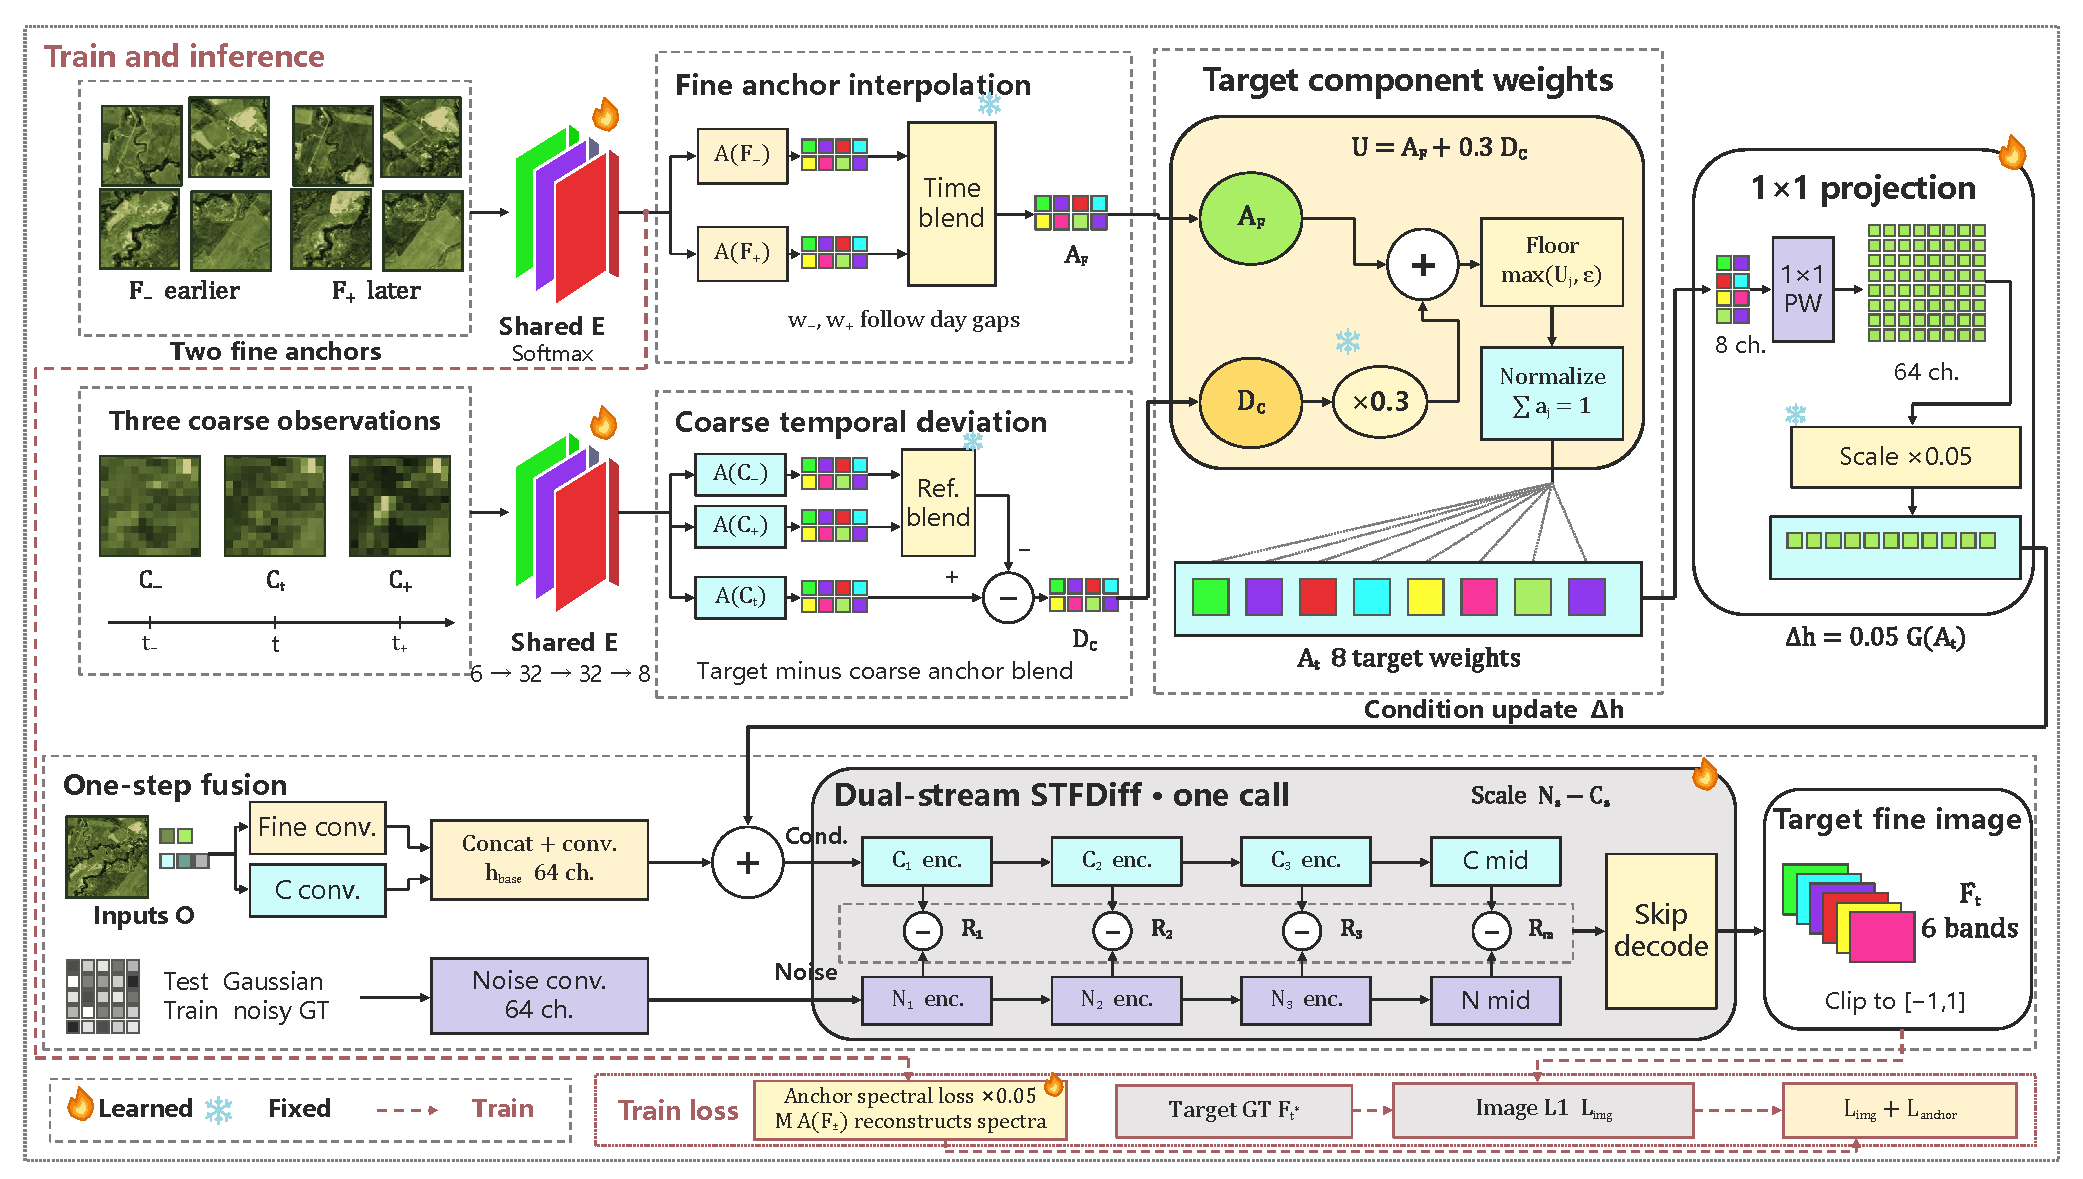
\includegraphics[width=\textwidth]{mechanism_en.pdf}
\caption{Dual-anchor component-weight correction and one-step reconstruction. The upper-left thumbnails show the five observations from one LGC patch. A shared encoder produces eight weights for each observation. The target-date coarse departure corrects the fine-reference weights. The pointwise projection adds $0.05G(A_t)$ to the conditioning stream. The backbone is evaluated once. Flames mark learned modules, snowflakes mark fixed operations, and dashed red paths carry training supervision.}
\label{fig:mechanism}
\end{figure*}

\section{Introduction}
Fine-resolution satellite imagery resolves land-surface boundaries, but a fine observation is often unavailable on the target date. More frequently acquired coarse observations provide evidence of change. Dual-anchor fusion estimates target-date fine reflectance from an earlier and a later fine image, paired coarse images, and a coarse observation on the target date. Flooding and vegetation growth can alter familiar structures, while several land-cover types may contribute to a single coarse pixel.

Conditional diffusion models such as STFDiff incorporate reference observations into the denoising process~\citep{huang2024stfdiff}. With one call to the denoiser, the conditioning pathway must provide both structural and temporal evidence within a limited inference budget. We ask whether explicitly encoding the target-date departure from the reference interpolation improves reconstruction. I10 uses a date-weighted fine blend as a starting point, transfers the coarse departure in a shared latent weight space, and projects the result into the original conditioning input. The design permits a paired comparison under a common backbone and number of evaluations.

We compare the selected checkpoint with a common 40-epoch endpoint for each of the 14 variants. Paired patch errors, latent-weight entropy and fixed-checkpoint interventions characterize the gain and the model's response to the coarse correction. The empirical study covers one LGC development date.

\section{Related work}
STARFM and FSDAF use available observations to model spatiotemporal change. FSDAF combines spectral unmixing and thin-plate splines to distribute coarse residuals~\citep{gao2006starfm,zhu2016fsdaf}. STFDiff learns a conditional distribution of fine images through diffusion~\citep{huang2024stfdiff}. SA-STF combines residual diffusion, temporal feature alignment and semantic-adaptive fusion~\citep{zhang2026sastf}. Its authors identify detail recovery under rare abrupt changes without matched references as an open problem. WPFM-STF starts from a learned spatiotemporal prior and uses a wavelet constraint during few-step flow matching~\citep{hu2026wpfm}. Its local analysis shows spatial residuals can persist after a patch-wide radiometric offset has been reduced.

Hyperspectral methods such as EndNet use nonnegative bases and component weights for spectral reconstruction~\citep{ozkan2019endnet}. I10 shares an eight-channel representation across sensors and dates. A learned basis supervises auxiliary reconstruction at the two fine anchors, and the one-step backbone produces the target fine prediction. A material interpretation of the component channels requires independent evidence.

\section{Method}
\subsection{Observations and one-step baseline}
Let $F_-$ and $F_+$ be the earlier and later fine references, with corresponding coarse observations $C_-$ and $C_+$. The target-date coarse image is $C_t$. The date gaps are $\Delta_-=t-t_-$ and $\Delta_+=t_+-t$. The input contains five six-band images on a common $256\times256$ grid and the two gaps. Images are scaled to $[-1,1]$, and $\reflectance(X)=(X+1)/2$ restores the reflectance domain.

The two streams of the baseline encode the observations and a noisy state. Separate convolutions process the fine and coarse observations. Concatenation and projection produce the 64-channel condition $h_{\mathrm{base}}$. At each resolution, the network subtracts the conditional features from the noisy features and passes the residuals to a decoder. The backbone uses the noise level and predicts the target fine image $\widehat F_t$.

\subsection{Latent-weight correction}
The shared encoder $E$ uses a $3\times3$ convolution, a depthwise $3\times3$ convolution and a $1\times1$ projection, with widths $6,32,32,8$. A channel-wise softmax produces the weight vector at position $p$.
\begin{equation}
 A(X,p)=\operatorname{softmax}_{j}\!\left[E(\reflectance(X))(p)\right].
 \label{eq:weights}
\end{equation}
The encoder is shared by all five images. Let $w_+=\Delta_-/(\Delta_-+\Delta_+)$ and $w_-=1-w_+$. Dropping the position index, we define the fine blend $A_F$ and the target-date coarse departure $D_C$ as
\begin{align}
 A_F &= w_-A(F_-)+w_+A(F_+),\\
 D_C &= A(C_t)-w_-A(C_-)-w_+A(C_+).
 \label{eq:coarse}
\end{align}
The correction is added in this shared space. The entries are floored at $10^{-6}$ and divided by their sum.
\begin{align}
 U&=A_F+0.3D_C,\\
 V_j&=\max(U_j,10^{-6}),\qquad
 A_{t,j}=\frac{V_j}{\sum_{\ell=1}^8 V_\ell}.
 \label{eq:transfer}
\end{align}
A learned $1\times1$ projection $G$ maps the eight weights to 64 channels. I10 uses $h_{\mathrm{base}}+0.05G(A_t)$ as the condition. Figure~\ref{fig:mechanism} shows where this update enters the shared backbone.

\subsection{Training and inference}
Training uses a 100-level cosine noise schedule~\citep{nichol2021improved}. For noise index $k$, the target fine image $\target$ and a standard Gaussian draw $\varepsilon$ define
\begin{equation}
 X_k=\sqrt{\bar\alpha_k}\target+\sqrt{1-\bar\alpha_k}\varepsilon.
\end{equation}
The target prediction is clipped to $[-1,1]$. During training, a shared basis $M=\operatorname{sigmoid}(\Theta)$, with $\Theta\in\mathbb R^{6\times8}$, also reconstructs each fine reference. The objective is
\begin{align}
 \mathcal L={}&\avg{|\widehat F_t-\target|}\\
 &+0.05\sum_{i\in\{-,+\}}
  \avg{|M A(F_i)-\reflectance(F_i)|},
 \label{eq:objective}
\end{align}
where angle brackets average bands and pixels. Inference initializes the state with standard Gaussian noise, evaluates the backbone once at $k=99$, and returns the clipped prediction. Both backbone configurations make one denoising call. I10 adds \ExtraParameters{} parameters and a conditioning computation to the \BaseParameters{}-parameter baseline.

\begin{table*}[!t]
\centering
\caption{Mean patch RMSE for all 30 from-scratch runs on the same LGC development split. Each seed has 15 runs. The best checkpoint is selected by validation RMSE. The common endpoint is epoch 40.}
\label{tab:main}
\small
\setlength{\tabcolsep}{12pt}
\begin{tabular}{lrrrr}
\toprule
& \multicolumn{2}{c}{Seed 42} & \multicolumn{2}{c}{Seed 123}\\
\cmidrule(lr){2-3}\cmidrule(lr){4-5}
Method & Best checkpoint & Epoch 40 & Best checkpoint & Epoch 40\\
\midrule
\PrimaryRows
\bottomrule
\end{tabular}
\end{table*}

\begin{figure*}[!t]
\centering
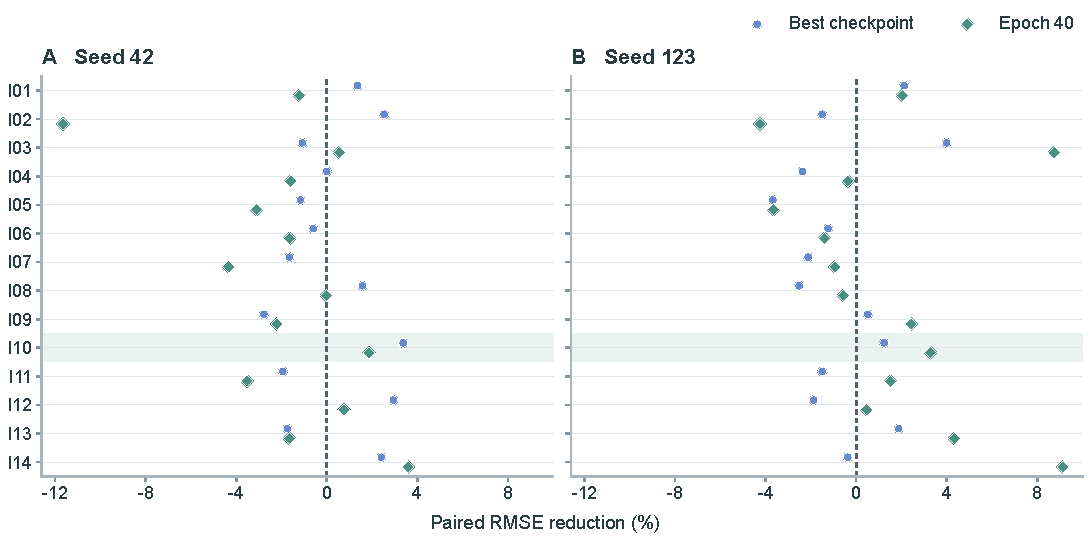
\includegraphics[width=.94\textwidth]{gains_en.pdf}
\caption{RMSE reductions relative to the paired baseline for the 14 variants. Circles denote each run's selected checkpoint. Diamonds denote epoch 40. Positive values indicate lower error.}
\label{fig:gains}
\end{figure*}

\section{Experimental protocol}
\subsection{Data, pairing and metrics}
The LGC Landsat--MODIS reflectance series is available from CSIRO~\citep{emelyanova2013blending,csiro2014lgc}. The frozen training split contains 1,200 patches from ten triples. The development split contains 120 nonoverlapping patches with target date 2 March 2005. Coarse images are co-registered on the common grid. Training triples exclude the validation target date. This scene has previously been used for project development.

The six-epoch screen fine-tunes the baseline and 14 variants from the same historical initialization. The from-scratch study trains all 15 configurations for 40 epochs at seeds 42 and 123. Runs within a seed share backbone initialization, sample order and base noise draws. Replication uses Adam with a peak learning rate of $2\times10^{-4}$, accumulation over two microbatches, and 600 optimizer updates per epoch. All runs use the common split and checkpoint rules.

Validation averages reflectance RMSE over 120 patches and three fixed noise draws per patch. The primary table reports each run's minimum-validation-RMSE checkpoint and the common epoch 40. Structural similarity (SSIM), spectral angle (SAM, in radians), ERGAS and the correlation coefficient (CC) are exported at the selected checkpoints.

\subsection{Paired patch analysis and interventions}
For each patch and checkpoint, we average the three noise realizations. We subtract the variant error from the baseline error at the matching seed. The validation grid forms 30 nonoverlapping $2\times2$ patch blocks. We take the $2.5$th and $97.5$th percentiles of 10,000 resampled block means. These intervals describe spatial variation within the development scene. We also group patches into tertiles of the mean absolute departure of $C_t$ from the date-weighted coarse anchor blend, with 40 patches in each group.

The fixed-checkpoint intervention uses two patches, one common noise draw per patch, and the seed 42 checkpoint at epoch 32. We compare the full model, zero coarse departure, spatially shuffled $32\times32$ departure blocks, and removal of the complete conditioning increment. The interventions measure the response of a trained model to these changes.

\begin{figure*}[!t]
\centering
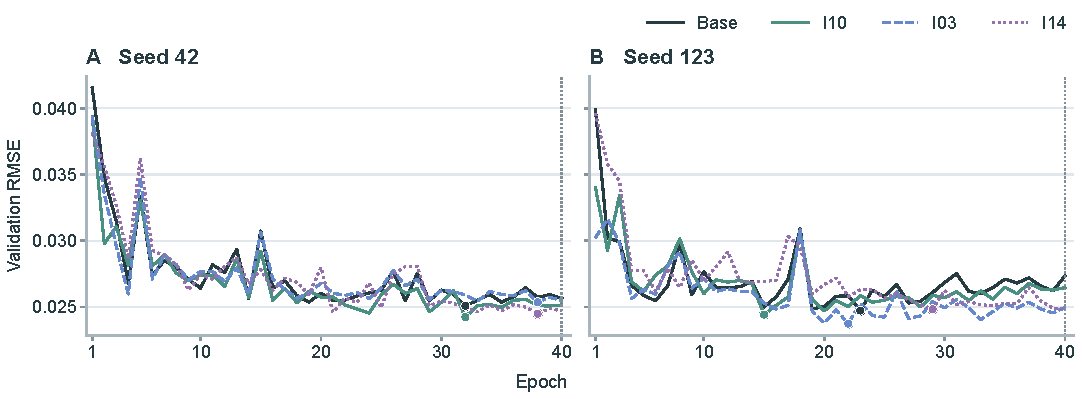
\includegraphics[width=.94\textwidth]{trajectory_en.pdf}
\caption{Validation trajectories for the baseline and representative variants. Dots mark each curve's minimum, and the vertical dotted line marks epoch 40. The archive retains every trajectory.}
\label{fig:trajectory}
\end{figure*}

\begin{figure*}[!t]
\centering
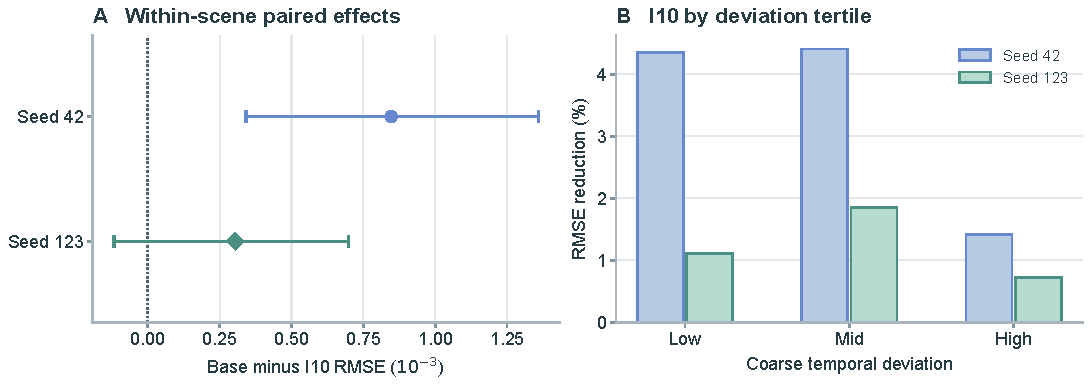
\includegraphics[width=.94\textwidth]{diagnostics_en.pdf}
\caption{I10 at the selected checkpoints. A reports paired RMSE differences (base minus I10) and bootstrap percentile intervals from spatial blocks within the scene. B shows the group RMSE reduction relative to the baseline in each of three coarse-deviation tertiles.}
\label{fig:diagnostics}
\end{figure*}

\section{Results}
\subsection{Rankings across seeds and checkpoints}
All 14 variants had higher best-checkpoint RMSE than the original-weight reference (\ScreenReference{}) in the warm-start screen. Relative performance changed under the 40-epoch from-scratch protocol. Table~\ref{tab:main} and Fig.~\ref{fig:gains} retain all comparisons.

At the selected checkpoints, I10 reduced RMSE from \BaseBestA{} to \MainBestA{} at seed 42 and from \BaseBestB{} to \MainBestB{} at seed 123. At epoch 40, it reduced RMSE from \BaseFinalA{} to \MainFinalA{} and from \BaseFinalB{} to \MainFinalB{}, respectively. I01 improved at the selected checkpoints of both seeds and had higher error at epoch 40 for seed 42. I03, I12 and I14 improved at epoch 40 for both seeds, with at least one seed reversing direction at the selected checkpoint. I14 attained the lowest epoch-40 RMSE in both seed blocks. I03 attained the lowest selected-checkpoint RMSE at seed 123. Figure~\ref{fig:trajectory} shows the corresponding trajectories.

\begin{table}[!t]
\centering
\caption{Secondary metrics for the baseline and I10 at the selected checkpoints. SAM is in radians.}
\label{tab:secondary}
\small
\setlength{\tabcolsep}{2.15pt}
\begin{tabular}{rlrrrrr}
\toprule
Seed & Method & Best epoch & SSIM $\uparrow$ & SAM $\downarrow$ & ERGAS $\downarrow$ & CC $\uparrow$\\
\midrule
\SecondaryRows
\bottomrule
\end{tabular}
\end{table}

\subsection{Spectral metrics and spatial distribution}
I10 lowered SAM and ERGAS at the best checkpoints of both seeds (Table~\ref{tab:secondary}). CC decreased slightly for both seeds. SSIM decreased slightly at seed 42 and increased at seed 123.

The mean paired RMSE reductions were \MeanPairA{} and \MeanPairB{} in units of $10^{-3}$, with lower errors in \BetterPatchesA{} and \BetterPatchesB{} of the 120 patches, respectively. The within-scene interval at seed 42 was $[\LowPairA,\HighPairA]\times10^{-3}$. At seed 123, the interval $[\LowPairB,\HighPairB]\times10^{-3}$ crossed zero (Fig.~\ref{fig:diagnostics}A). Group-mean RMSE decreased in every coarse-deviation tertile, with the smallest reductions in the highest tertile for each seed (Fig.~\ref{fig:diagnostics}B). The strata describe the departure from the coarse reference blend. Fine-scale change type and location require dedicated labels or diagnostics.

\subsection{Latent weights and response to the coarse departure}
For both I10 checkpoints, the median of the patch-averaged entropy was approximately $1.037\times10^{-4}$ nat. This is close to the entropy of a single-channel assignment after the floor and normalization in Eq.~\eqref{eq:transfer}. The concentration motivates checking channel occupancy and projection amplitude before interpreting the learned weights.

On the two intervention patches, the full I10 model had RMSE \ProbeFull{}. Zeroing and shuffling $D_C$ yielded \ProbeZero{} and \ProbeShuffle{}, respectively. Removing the entire conditioning increment yielded \ProbeNoInjection{}, and the baseline yielded \ProbeBase{}. These patches show different sensitivities to the full increment and its target-date correction. A full-scene intervention and matched retraining are needed to establish the effect of the correction.

\section{Discussion}
The paired results motivate keeping I10 for further diagnosis and retaining I03 and I14 as informative endpoint controls. The rankings illustrate how the selection rule changes the interpretation of each variant. I10 reduced RMSE under both rules, while the spatial intervals and interventions delimit the scope of this observation.

The concentration in both checkpoints and the near-zero response to the coarse departure in the small intervention leave open the source of the gain. A full set of fixed-weight interventions should be paired with from-scratch controls that remove the departure, learn a constant condition or use a capacity-matched raw-reflectance residual. These comparisons test how much the temporal and spatial information contributes to reconstruction.

A common-protocol external comparison should reproduce a strong five-observation method and compare its native and modified versions under a shared training split and evaluation. The original SA-STF training dates include our development target date, which constrains the use of its released weights here~\citep{zhang2026sastf}. Independent dates and regions can then test localization of fine-scale change, false changes in stable areas and end-to-end inference cost.

\section{Conclusion}
Across 30 from-scratch runs on one development date, I10 reduced the one-step STFDiff baseline's validation RMSE at the selected checkpoints and at epoch 40 for both seeds. The concentrated weights and the small intervention motivate testing the contribution of the temporal correction directly. Held-out change recovery and a common-protocol comparison with stronger external methods are the next confirmation steps.

\section*{Code and experiment records}
The archive supplies configurations, epoch logs, per-patch metrics, source snapshots, checkpoints and the scripts used to reproduce the displays for the screening runs and the two-seed replication. \href{https://github.com/qing1989620/paper-shikongyaogan/releases/tag/stf-stage-20261125}{GitHub release and checksums}

\FloatBarrier
\balance
\bibliographystyle{IEEEbib}
\bibliography{refs}
\end{document}
